% -----------------------------------------
\chapter{Projeto e Desenvolvimento}\label{chp:LABEL_CHP_4}
% -----------------------------------------
Nesta seção são detalhados os passos e decisões tomadas ao decorrer do período de desenvolvimento deste trabalho. São apresentadas as etapas de implementação e integração com outras soluções utilizadas, assim como a execução e comparação dos resultados obtidos.

\section{Casos de uso}
Inicialmente foi desenvolvido o caso de uso expandido do sistema, baseando-se no que foi demonstrado por \citeonline{SOMMERVILE} do modelo UML, como forma tanto de documentação, assim como planejamento do protótipo. Por meio destes, todas as interações do sistema com seus usuários foram pré-determinadas, assim como a definição e organização de requisitos funcionais no sistema dado seu contexto para modelagem do fluxo básico dos eventos diretamente nestes diagramas.

Além disto, o caso de uso, mostra neste contexto o escopo da aplicação, trazendo as principais funcionalidades que foram desenvolvidas no protótipo limitando-se a eventos educacionais online. Adicionando a isto, os cenários de interação entre os atores por meio do caso de uso determinado definem principalmente como deveria ser planejado e até qual ponto pode ser utilizado por cada um deles, respeitando sua hierarquia. 

Com base neste diagrama, e sua devida explicação foi possível traçar uma rota de desenvolvimento por meio do processo unificado. No início foi pensado em apenas dois atores, sendo estes um administrador e um usuário comum, como mostra a imagem. Nisto, foram desenvolvidas funcionalidades básicas para estes, contendo a primeira iteração, sem os demais. \\
Seguindo em frente, para a segunda iteração, já há mais atores contando com a inclusão do associado, sendo intermediário entre usuário e supervisor. Além disso, e novas funcionalidades pensadas para a aplicação, sendo estas a gerência da lista de participantes e a gerência dos eventos apenas para determinado usuários (sendo estas relacionadas ao associado).
Na terceira iteração foram identificadas necessidades de atores que não precisavam necessariamente de um login como é o caso do visitante, que poderá apenas visualizar os eventos e validar certificados, que são operações mais simples e que não necessitam de qualquer permissão especial. 

Na quarta e última iteração até o momento o sistema está mais moldado pensando em diversas funcionalidades, inclusive com o caso de uso expandido, tendo em vista melhor as funcionalidades e seus retornos do sistema para o ator determinado.

\section{Mokcups}
Dados os casos de uso, será possível criar um mockup das telas baseado nestas informações. Ou seja, a criação de telas por meio do Figma possibilitou a visualização e alteração do layout de uma forma simplificada antes de serem implementadas de fato. Dito isso, toda o mockup foi pensado para seguir padrões na interface, como por exemplo a barra de navegação está presente em todas as páginas a qual o usuário poderá navegar (com exceções apenas da criação de conta e login). E isto facilita a navegação, e mantém a similaridade da aplicação para o usuário final.  

A figura \ref{home_mockup} demonstra como é a ideia da página inicial, que contém uma barra de navegação, um acesso aos eventos, um acesso a criação de eventos e ao perfil. Haverá, no meio da página, um destaque aos últimos eventos cadastrados na plataforma, podendo ser acessados diretamente desta página.
\begin{figure}[h]
    \caption{\label{home_mockup}Mockup da tela inicial}
    \vspace{5pt}
    \centering
    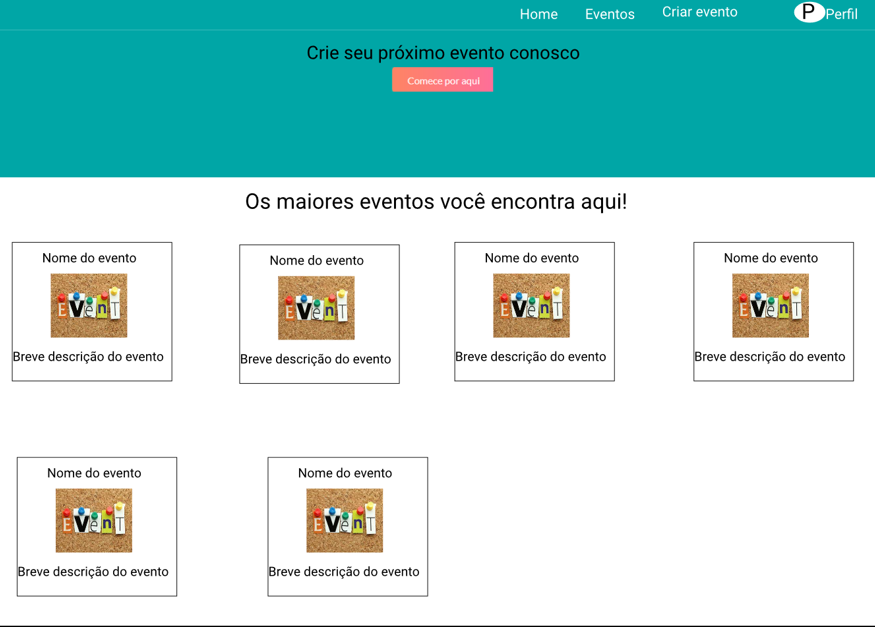
\includegraphics[scale=.4]{home_mockup.png}
    \vspace{5pt}
    \legend{Fonte: Próprio autor}
\end{figure}

Para a página seguinte, a figura \ref{evento_mockup} mostra como é a visualização detalhada de um evento, com sua descrição, imagem e suas atividades cadastradas. Estes detalhes são os compostos especificamente para um evento, mas a barra de navegação citada anteriormente na página inicial estará presente para facilitar a navegação entre páginas.
\begin{figure}[h]
    \caption{\label{evento_mockup}Mockup da tela do evento}
    \vspace{5pt}
    \centering
    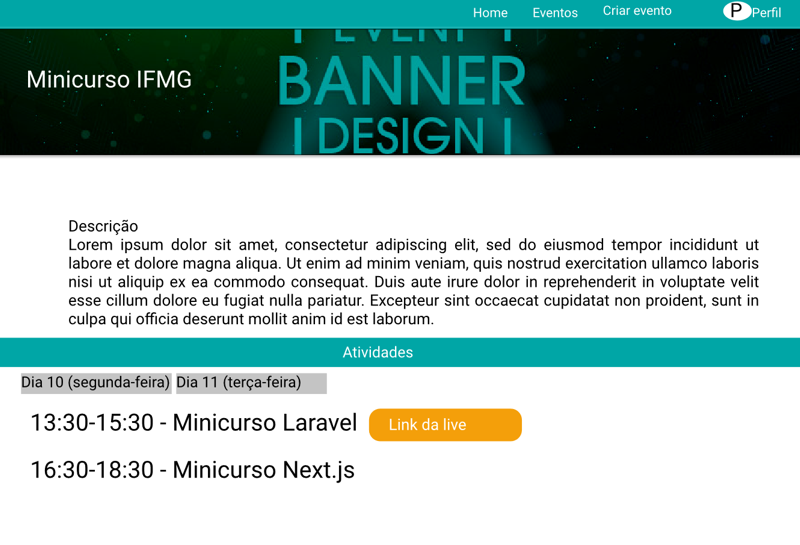
\includegraphics[scale=.4]{evento_mockup.png}
    \vspace{5pt}
    \legend{Fonte: Próprio autor}
\end{figure}

A terceira parte do mockup é a tela de pesquisa de eventos, como mostra a figura \ref{pesquisa_mockup}, que assim como as demais mantém a barra de navegação para facilitar o acesso e possui diversos filtros para os eventos. Estes filtros definidos por categoria, instituição, data inicial e final e horário inicial e final, foram definidos como os principais para a pesquisa. E ao final da página, percebe-se a paginação, ou seja, caso passe de uma determinada quantidade, serão criadas diversas abas possíveis da mesma pesquisa.
\begin{figure}[h]
    \caption{\label{pesquisa_mockup}Mockup da tela de pesquisa}
    \vspace{5pt}
    \centering
    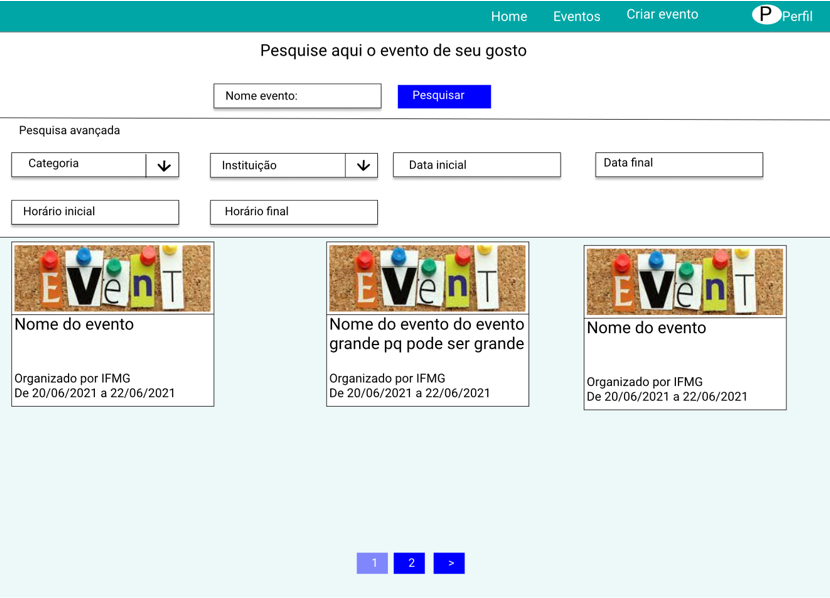
\includegraphics[scale=.4]{pesquisa_mockup.png}
    \vspace{5pt}
    \legend{Fonte: Próprio autor}
\end{figure}

Por fim, a figura \ref{form_mockup}, mostra como serão todos os formulários do sistema, sendo este utilizado de acordo com a necessidade da tela, como a criação de eventos ou criação de usuário. Isto se deve para melhorar tal interação, tornando padronizado e fazendo com que não seja necessário retrabalho de aprendizagem para cada página contida.
\begin{figure}[h]
    \caption{\label{form_mockup}Mockup da tela de formulário padrão}
    \vspace{5pt}
    \centering
    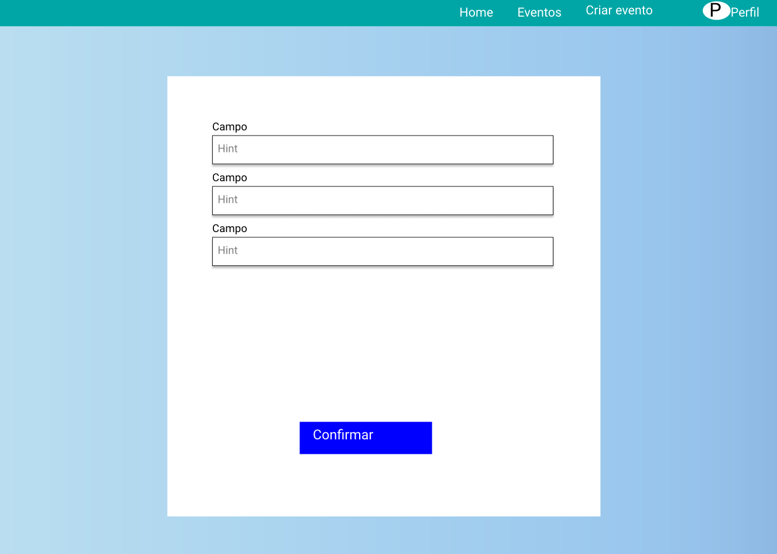
\includegraphics[scale=.4]{form_mockup.png}
    \vspace{5pt}
    \legend{Fonte: Próprio autor}
\end{figure}

Com todas estas informações sobre a responsabilidade e design de cada tela da aplicação, é possível a criação de maneira estruturada, além de padronizada da interface para o usuário. 

\section{Estruturação}
A estruturação segue um modelo de distribuição vertical, o qual prevê a distinção entre divisão de componentes, neste caso a interface com o usuário e a API, em dois servidores distintos, sendo um alocado na Vercel e outro no Heroku. Mesmo que uma aplicação dependa da outra para que funcione integralmente, são serviços distintos e que melhoram de maneira geral o funcionamento do sistema, visto que tais responsabilidades distintas melhoram o tempo de carregamento. Ou seja, enquanto back-end persiste os dados e os processa diretamente, respondendo a requisições, o front-end fará as requisições recuperando o arquivo JSON gerado e o transformando em uma interface gráfica tangível ao usuário.


\section{Modelos}
Nesta etapa, foram criados modelos os quais tiveram embasamento no diagrama de Caso de Uso, assim como nos mockups, visto que deve atender os requisitos predeterminados. Desta forma, foram criados os modelos conforme figura \ref{modelo_banco}, que determina cada classe do banco de dados feita no Laravel para que possa representar os relacionamentos entre as tabelas do MySQL, além de determinar cada atributo das classes. Estes foram feitos com base na figura \ref{models_projeto}, que representa o diagrama de entidade e relacionamento do banco de dados.
\begin{figure}[h]
    \caption{\label{modelo_banco}DER do banco de dados}
    \vspace{5pt}
    \centering
    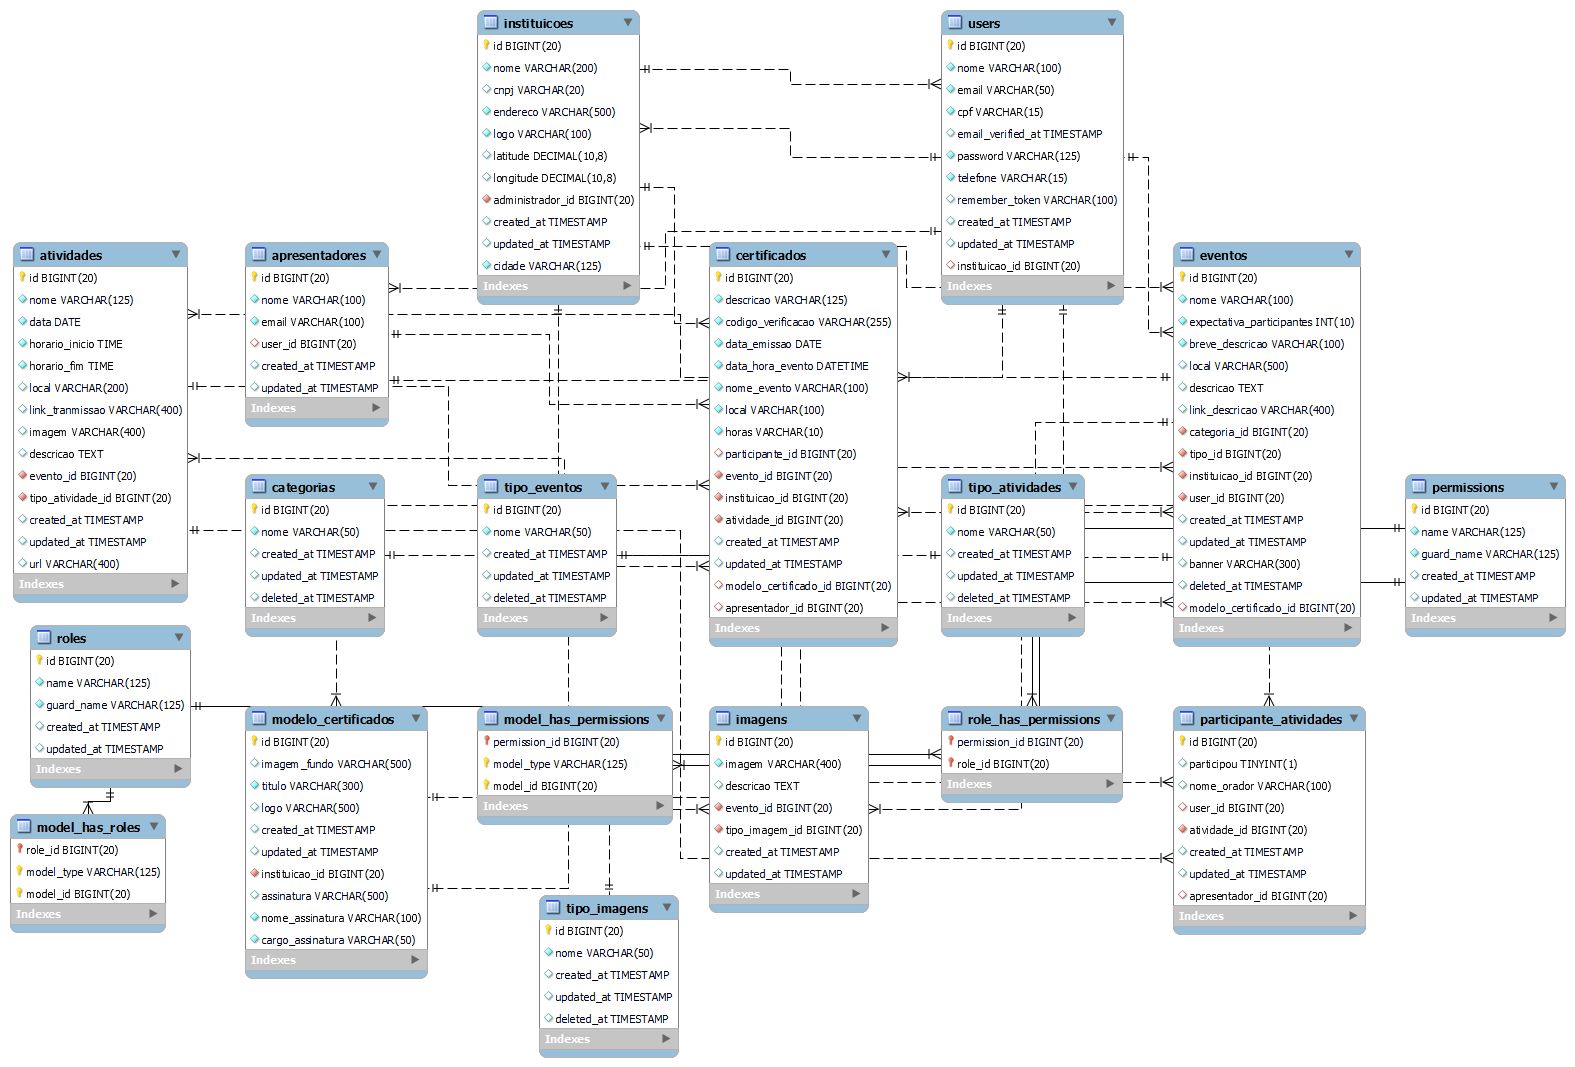
\includegraphics[scale=.25]{modelo_banco.png}
    \vspace{5pt}
    \legend{Fonte: Próprio autor}
\end{figure}
\begin{figure}[h]
    \caption{\label{models_projeto}Classes de modelo}
    \vspace{5pt}
    \centering
    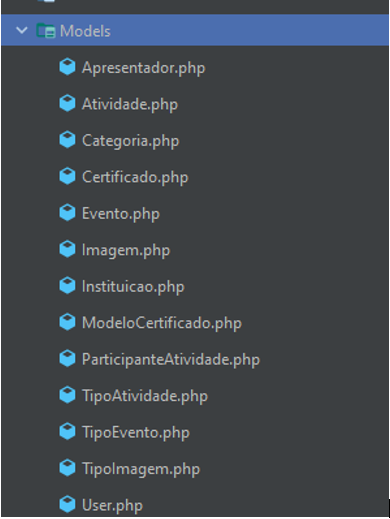
\includegraphics[scale=.5]{models_projeto.png}
    \vspace{5pt}
    \legend{Fonte: Próprio autor}
\end{figure}

\section{Controllers}
Por meio dos controladores do Laravel, é possível manipular as operações do banco de dados, e para que haja uma organização e mantenha o padrão MVC, foram criados controladores específicos para cada modelo, sendo cada um atribuído a responsabilidade do modelo correspondente e essa estruturação pode ser vista na figura \ref{controllers}, a qual demonstra cada um dos controladores.
\begin{figure}[h]
    \caption{\label{controllers}Controladores}
    \vspace{5pt}
    \centering
    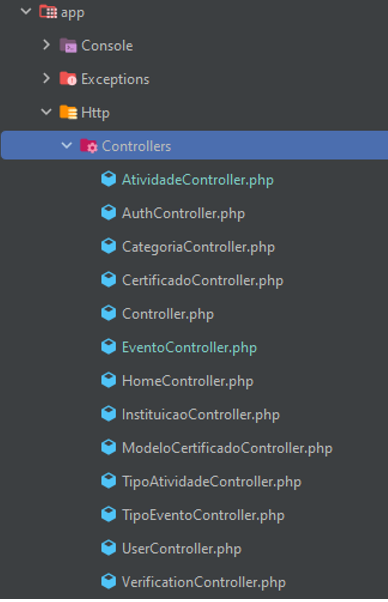
\includegraphics[scale=.5]{controllers.png}
    \vspace{5pt}
    \legend{Fonte: Próprio autor}
\end{figure}

Além disso, por fazerem parte de uma API (explicada com mais detalhes posteriormente), cada operação deve retornar um JSON, juntamente com o código de status de retorno do HTTP. No trecho de código, visto na figura \ref{orm}, é um exemplo da função a qual recebe uma requisição determinando cada um dos filtros, e então por meio do eloquent ORM, realizando a query no banco de dados e no fim retornando um JSON com os dados, padronizando, então, a maneira de se receber e retornar os dados.
\begin{figure}[h]
    \caption{\label{orm}Exemplo do ORM}
    \vspace{5pt}
    \centering
    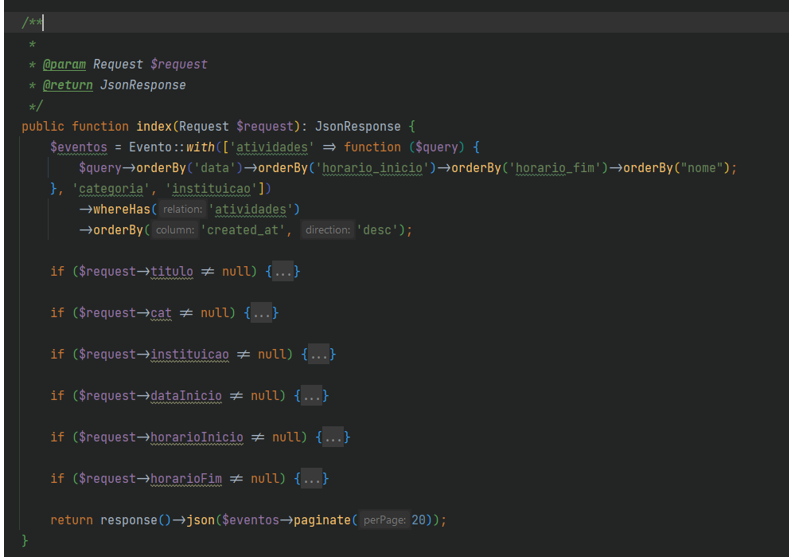
\includegraphics[scale=.5]{ORM.png}
    \vspace{5pt}
    \legend{Fonte: Próprio autor}
\end{figure}

Dado o exemplo da busca e seus filtros, a validação de dados na inserção e atualização de dados é essencial para que não haja dados inseridos de maneira indevida e que haja um padrão nas requisições. Isto tudo é feito diretamente no Laravel, que validará antes mesmo do banco de dados e retornará caso haja algum erro.
\section{Operações API}
A API foi feita no Laravel, respeitando os padrões estabelecidos pela interface REST. Ou seja, por meio de requisições HTTP do tipo GET, POST e DELETE é possível acessar todas as rotas do back-end. Em diversas destas não será possível acessar sem que haja uma autenticação feita por meio do JWT, que irá validar se há permissão de acesso, e isto determina caso o usuário esteja logado, assim como seu nível de acesso dentro de sua hierarquia. 

Dito isso, as rotas foram criadas em grupos para atenderem as necessidades e criar-se uma organização para cada requisição, então foram organizadas, conforme a figura \ref{rotas_laravel}. Esta demonstra cada um dos agrupamentos, sendo estes aqueles que contém todas as rotas para modelos, assim como para determinadas funcionalidades do sistema. O grupo de eventos terá todas as rotas pertencentes a eventos, sendo estas demonstradas na figura \ref{grupo_rotas}, e conforme pode ser visualizado possuem autenticação e validação do que pode ser escrito na url para que possa ser acessada devidamente. 
\begin{figure}[h]
    \caption{\label{rotas_laravel}Grupo de rotas}
    \vspace{5pt}
    \centering
    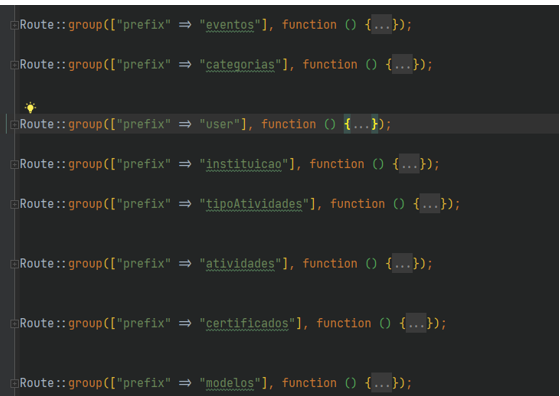
\includegraphics[scale=.3]{rotas_laravel.png}
    \vspace{5pt}
    \legend{Fonte: Próprio autor}
\end{figure}
\begin{figure}[h]
    \caption{\label{grupo_rotas}Exemplo grupo de rotas}
    \vspace{5pt}
    \centering
    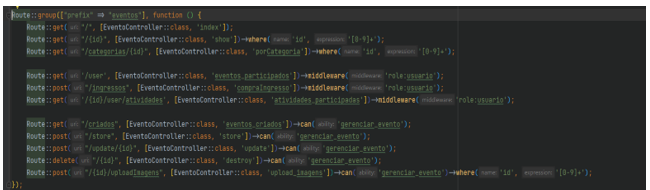
\includegraphics[scale=.5]{grupo_rotas.png}
    \vspace{5pt}
    \legend{Fonte: Próprio autor}
\end{figure}

\section{Componentes}
Diferentemente do webservice criado no Laravel, a estruturação do frontend no Next.js é feito por meio de componentes, e por ter utilizado do Typescript, há também os tipos que irão fornecer um auxílio no momento da transcrição dos dados, seja na requisição quanto na resposta da API. Na figura \ref{estrutura_next} é possível ver a estruturação geral do projeto, sendo dividido em componentes, páginas, imagens, tipos, utilitários e a configuração do Firebase.
\begin{figure}[h]
    \caption{\label{estrutura_next}Estrutura do projeto do Next.js}
    \vspace{5pt}
    \centering
    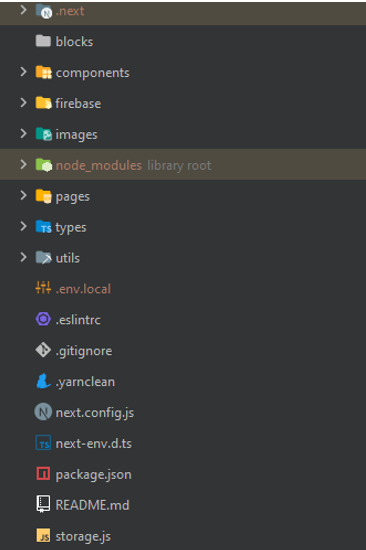
\includegraphics[scale=.35]{estrutura_next.png}
    \vspace{5pt}
    \legend{Fonte: Próprio autor}
\end{figure}

Por meio dos componentes, mostrados na estrutura da figura \ref{componentes} é possível a reutilização do código-fonte para diversos layouts, como por exemplo o componente NavBar, o qual é utilizado em diversas páginas, tornando-as padronizadas. Com isto, cada componente, também, terá seu estilo por meio de um arquivo de módulo do CSS, que estende os estilos globais, podendo sobrepô-los. Portanto, cada componente terá sua finalidade pré-definida, podendo ser reutilizada caso sirva o propósito.
\begin{figure}[h]
    \caption{\label{componentes}Estrutura dos componentes}
    \vspace{5pt}
    \centering
    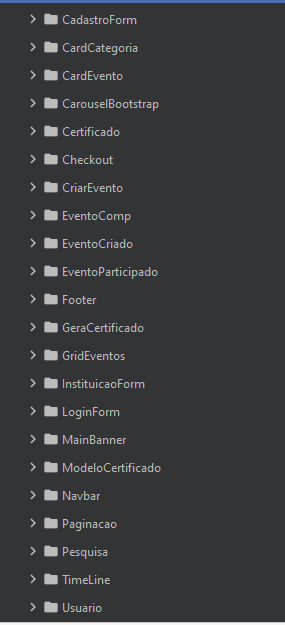
\includegraphics[scale=.4]{componentes.png}
    \vspace{5pt}
    \legend{Fonte: Próprio autor}
\end{figure}


\section{Rotas Next.js}
Em relação as rotas, serão as páginas a serem acessadas pelo usuário. Dito isso, estas deverão validar, caso necessário, se o usuário está logado por meio de uma requisição ao back-end. Além disso, estas devem requisitar diversas informações para que possam ser exibidas nas páginas e preencherem os dados necessários de cada componente. Conforme estruturação presente na figura \ref{pages}, cada página tem seu nome e sua estruturação interna, podendo ter sub-rotas, que serão chamadas dentro da pasta. Esta regra vale para todas as pastas presentes, com exceção das 404 (a qual está destinada a páginas não encontradas, ou seja, caso seja digitada uma url dentro do domínio que não seja pertencente a esta lista, irá a chamar, visto que é uma página customizada) e a 403 (que determina um recurso não possível de ser acessado para determinado usuário).
\begin{figure}[h]
    \caption{\label{pages}Estruturação de páginas no Next.js}
    \vspace{5pt}
    \centering
    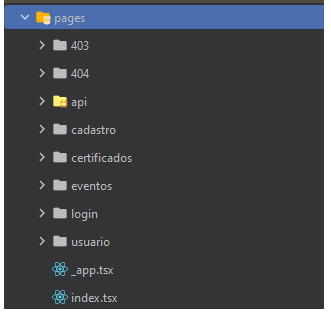
\includegraphics[scale=.4]{pages.png}
    \vspace{5pt}
    \legend{Fonte: Próprio autor}
\end{figure}

\section{Renderização das páginas}
Dentro das páginas da aplicação, diretamente do Next.js, foram utilizadas ambas as implementações de pré-renderização presentes no framework. Em páginas que podem ter cache, como por exemplo, as páginas individuais de cada evento, principalmente por conterem diversas imagens, além de não necessariamente precisarem estar constantemente sendo atualizadas, sendo estas geradas em tempo de compilação, e tendo em vista que o evento nem seja editado, foi utilizado o método de Static Generation com Incremental Static Regeneration. Ou seja, por todas as páginas serem baseadas nos mesmos componentes, tendo sua diferença apenas os dados requisitados, foi criado um cache para cada um, gerando uma página HTML juntamente com um JSON de dados, para cada das páginas. Isto faz com que o acesso seja mais rápido, e o cache é de um minuto, ou seja, a cada um minuto se o evento for editado e caso haja uma requisição, a página será gerada novamente com base no que foi atualizado em cada uma das páginas desta rota dinâmica.

Além disso, há também a outra implementação de pré-renderização, que é a Server-side rendering, que foi utilizada em páginas, como a de pesquisa dos eventos. A sua utilização se deve ao fato de que esta deve ser geradas constantemente baseada nos filtros que o usuário irá fazer dada a sua necessidade. A página é mais lenta em relação a uma geração estática, porém todo o processamento fica no servidor que está hospedada a aplicação, deixando com o navegador do usuário final apenas com o HTML gerado em tempo de execução dada essa frequência de atualização desta página, por exemplo.
